% ------------------------------------------------------------
% File: figures/fig-interleaved-quadrants.tex
% Interleaved recess depths across two samples with quadrant-mask inset
% ------------------------------------------------------------

\begin{figure}[htbp]
  \centering
  \begin{tikzpicture}[x=0.8cm, y=0.8cm, font=\footnotesize]
    % Parameters
    \def\cell{1.6}
    \def\vgap{1.25}
    \def\labely{-0.3}

    % Sample A and B (right), vertically centred against the inset.
    \begin{scope}[shift={(0,-1.2)}]
      \fill[gray!10] (0,\cell) rectangle (\cell,2*\cell);
      \fill[gray!30] (\cell,\cell) rectangle (2*\cell,2*\cell);
      \fill[gray!50] (0,0) rectangle (\cell,\cell);
      \fill[gray!70] (\cell,0) rectangle (2*\cell,\cell);
      \draw[line width=0.6pt] (0,0) rectangle (2*\cell,2*\cell);
      \draw[line width=0.6pt] (\cell,0) -- (\cell,2*\cell);
      \draw[line width=0.6pt] (0,\cell) -- (2*\cell,\cell);
      \node at (0.5*\cell,1.5*\cell) {10 nm};
      \node at (1.5*\cell,1.5*\cell) {20 nm};
      \node at (0.5*\cell,0.5*\cell) {30 nm};
      \node at (1.5*\cell,0.5*\cell) {40 nm};
      \node[anchor=north] at (\cell,\labely) {Sample A};

      % Highlight one repeated quadrant unit.
      \coordinate (zoomNW) at (0.12,2*\cell-0.12);
      \coordinate (zoomNE) at (\cell-0.12,2*\cell-0.12);
      \coordinate (zoomSW) at (0.12,\cell+0.12);
      \coordinate (zoomSE) at (\cell-0.12,\cell+0.12);
      \draw[red!75!black, dashed, line width=0.7pt] (zoomNW) rectangle (zoomSE);

    % Sample B (below)
    \begin{scope}[shift={(0,{-2*\cell-\vgap})}]
      \fill[gray!20] (0,\cell) rectangle (\cell,2*\cell);
      \fill[gray!40] (\cell,\cell) rectangle (2*\cell,2*\cell);
      \fill[gray!60] (0,0) rectangle (\cell,\cell);
      \fill[gray!80] (\cell,0) rectangle (2*\cell,\cell);
      \draw[line width=0.6pt] (0,0) rectangle (2*\cell,2*\cell);
      \draw[line width=0.6pt] (\cell,0) -- (\cell,2*\cell);
      \draw[line width=0.6pt] (0,\cell) -- (2*\cell,\cell);
      \node at (0.5*\cell,1.5*\cell) {15 nm};
      \node at (1.5*\cell,1.5*\cell) {25 nm};
      \node at (0.5*\cell,0.5*\cell) {35 nm};
      \node at (1.5*\cell,0.5*\cell) {45 nm};
      \node[anchor=north] at (\cell,\labely) {Sample B};
    \end{scope}
    \end{scope}

    % Zoomed quadrant mask inset.
    \node[
      anchor=east,
      draw,
      red!75!black,
      dashed,
      line width=0.7pt,
      inner sep=3pt
    ] (quadmask) at (-0.75,-1.75) {
      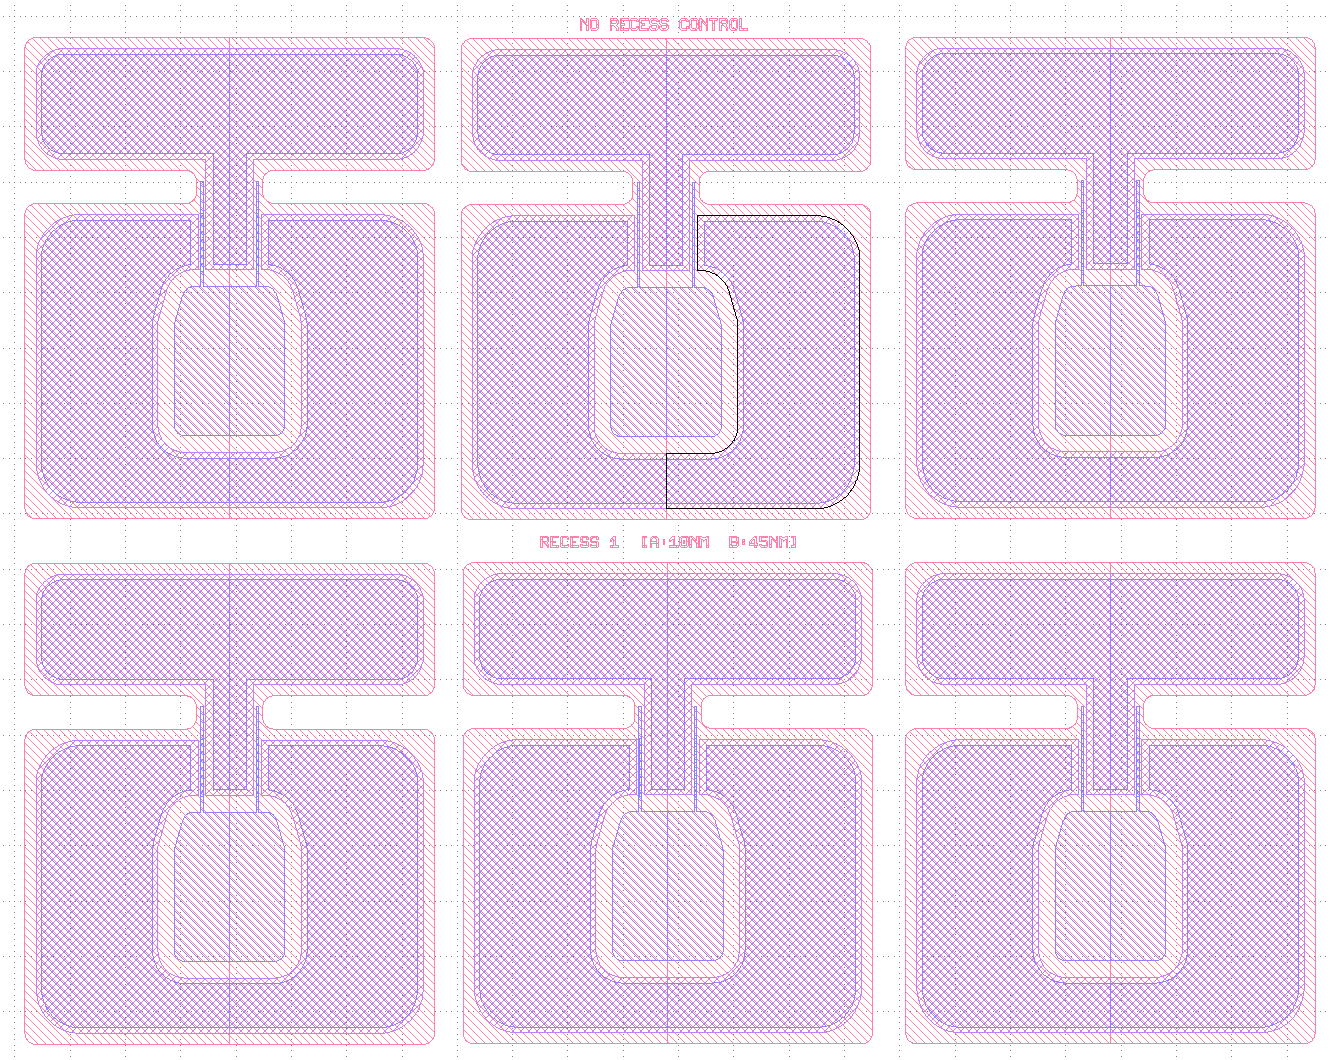
\includegraphics[width=12.3cm]{figures/gate_recession/quad_mask.png}
    };

    % Approximate control-device highlight: top row, second column.
    \coordinate (controlSW) at
      ($(quadmask.south west)!0.34!(quadmask.south east)
        +(0,0.40*12.3cm)$);
    \coordinate (controlNE) at
      ($(quadmask.south west)!0.66!(quadmask.south east)
        +(0,0.79*12.3cm)$);
    \draw[green!55!black, dashed, line width=2pt]
      (controlSW) rectangle (controlNE);
    \node[
      font=\small\bfseries,
      text=green!40!black,
      fill=white,
      fill opacity=0.75,
      text opacity=1,
      inner sep=1.5pt
    ] at ($(controlSW)!0.5!(controlNE)$) {Control Device};

    \begin{pgfonlayer}{background}
      \draw[red!75!black, dashed, line width=0.6pt]
        (zoomNW) -- (quadmask.north west);
      \draw[red!75!black, dashed, line width=0.6pt]
        (zoomNE) -- (quadmask.north east);
      \draw[red!75!black, dashed, line width=0.6pt]
        (zoomSW) -- (quadmask.south west);
    \end{pgfonlayer}

    \draw[red!75!black, dashed, line width=0.6pt]
      (zoomSE) -- (quadmask.south east);
  \end{tikzpicture}

  \vspace{2mm}
  \caption{Interleaved allocation of recess depths across two samples, with
  each quadrant containing the repeated set of five recessed devices and one
  unrecessed control device.}
  \label{fig:interleaved_quadrants}
  \label{fig:enhancement_mode_mask_quad}
\end{figure}
